\chapter{Confluencia}

En este capítulo estudiaremos el problema de determinar si un sistema
de reescritura es confluente. En la primera sección vamos a demostrar
que este problema es indecidible, sin embargo en las secciones
posteriores, estudiaremos que si el sistema es terminante, entonces el
problema es decidible. Por último veremos que ocurre para el caso de
los sistemas que no terminan.

\section{Estudio sobre el problema de decisión}
  
En esta sección veremos la indecibilidad para comprobar si un sistema
es confluente mediante el siguiente resultado,

\begin{teor}
  El problema de decidir si un sistema de reescritura finito $R$ es
  confluente, es indecidible.
\end{teor}

\begin{demo}
  El objetivo de esta demostración es reducir el problema de las
  palabras básicas para $E$ (que sabemos que es indecidible), a un
  sistema de reescritura de términos.

  Sea un conjunto de identidades $E$ tal que $\Var(l) = \Var(r)$ para
  todo $l \approx r \in E$. Sea $R := E \cup E^{-1}$, entonces al
  tener $\rightarrow_R = \leftrightarrow_E$ es confluente. Además $R$
  es un sistema de reescritura (por $\Var(l) = \Var(r)$).

  Dados dos términos básicos $s$ y $t$, y una constante $a$, vamos a
  probar que $R_{st} := R \cup \{ a \rightarrow s, a \rightarrow t \}$
  es confluente syss $s \approx_E t$.

  \begin{itemize}
  \item $(\Rightarrow)$ Si $R_{st}$ es confluente, entonces ni $s$, ni
    $t$ poseen una constante $a$, luego $s \downarrow_{R_{st}} t$. Esto
    significa que las reglas $a \rightarrow s, a \rightarrow t$ no
    pueden ser usadas. Por tanto $\rightarrow_R = \leftrightarrow_E$ y
    $s \approx_E t$.

  \item $(\Rightarrow)$ Vamos a probar que para términos $u, v$, si
    $u \rightarrow_{R_{st}} v$ entonces $v^t \xrightarrow{*}_R u^t$,
    donde $u^t$ denota el resultado de sustituir las constantes $a$ en
    $u$ por $t$.

    Supongamos que $u \rightarrow_{R{_st}} v$. Distinguimos que reglas
    se usan.
    \begin{itemize}
    \item Si usamos $u \rightarrow_R v$, reemplazamos $a$ por $t$ para
      conseguir $u^t \rightarrow_R v^t$ y por tanto
      $v^t \rightarrow_R u^t$ al ser $R$ simétrico.
    \item Si usamos $a \rightarrow s$, entonces $u|_p = a$ y
      $v = u[s]_p$ para alguna posición $p$. Como $s \approx_E t$
      entonces $s \xrightarrow{*}_R t$. Obtenemos
      $v \xrightarrow{*}_R u[t]_p$ que conlleva a
      $v^t \xrightarrow{*}_R (u[t]_p)^t$. Pero $(u[t]_p)^t =
      u^t[t^t]_p = u^t[t]_p = u^t$.
    \item Si usamos $a \rightarrow t$ en la posición $p$, entonces
      $v^t = (u[t]_p)^t = u^t \xrightarrow{*}_R u^t$.
    \end{itemize}
    Por tanto, si $u \xrightarrow{*}_{R_{st}} u_i$, para $i= 1,2$,
    entonces $u_i \xrightarrow{*}_{R_{st}} u_i^t \xrightarrow{*}_R u^t$
    y obtenemos $u_1 \downarrow_{R_{st}}$
  \end{itemize}
\end{demo}

\section{Pares críticos}

En esta sección estudiaremos la decibilidad para sistemas de
reescritura finitos que sean localmente confluentes.

La necesidad de los pares críticos surge de la importancia a la hora
de aplicar las reglas de un sistema de reescritura. Para entender
mejor este concepto, plantearemos el siguiente ejemplo. Sea $s$ un
término, $R := \{ l_1 \rightarrow r_1, l_2 \rightarrow r_2 \}$ donde
$l_1, l_2$ son subtérminos de $s$. Según apliquemos la primera regla o
la segunda, obtendremos un nuevo término $t$.

\begin{figure}[h]
  \centering
  \begin{tikzpicture}[->,>=stealth',level/.style={sibling distance =
      5cm/#1, level distance = 1.5cm}]

\node{$s$}
    child {
      node[align=center]{$t_1$}
        edge from parent node[above left] {$l_1 \rightarrow r_1$}}
    child {
      node{$t_2$}
      edge from parent node[above right] {$l_2 \rightarrow r_2$}
    };
\end{tikzpicture}
\end{figure}

Sea $p_i$ las posiciones y $\sigma_i$ las sustituciones tal que
$s|_{p_i} = \sigma_i l_i$ y $t_i = s[\sigma_i r_i ]_{p_i}, i
=1,2$. Tenemos que estudiar como de relacionados estan $p_1$ y $p_2$.

\begin{itemize}
\item Caso 1, $p_1$ y $p_2$ estan en árboles separados. En este caso,
  de da la convergencia local.

  % FALTA UNIR LOS 4 PRIMEROS EN UN ARBOL
  % AÑADIR COLOR
  % POSICIONAR MEJOR LOS SUBINDICES
  % FALTA POR ESCRIBIR UN GRAFICO
  % AÑADIR DESCRIPCIONES DE CADA UNO
  
  \centering
\begin{tikzpicture}
\draw (0,0) node[anchor=north]{}
  -- (10,0) node[anchor=north]{}
  -- (5,5) node[below]{$s$}
  -- cycle
   (2,0) node[anchor=north]{}
  -- (4,0) node[anchor=north]{}
  -- (3,1) node[below]{$\sigma_1 l_1$}
  -- cycle
     (8,0) node[anchor=north]{}
  -- (6,0) node[anchor=north]{}
  -- (7,1) node[below]{$\sigma_2 l_2$}
  -- cycle
  ;
\end{tikzpicture}

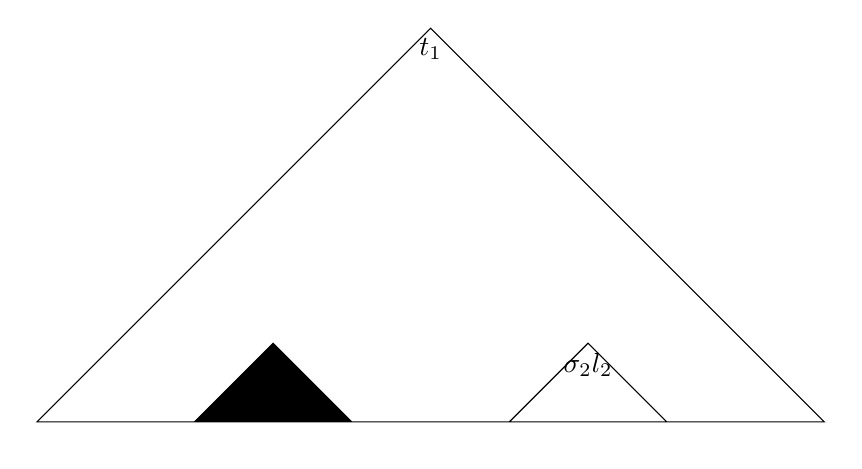
\begin{tikzpicture}
\node(a) at (2,0) {};
\node (b) at (4,0) {};
\node (c) at (3,1) {};

\draw (0,0) node[anchor=north]{}
  -- (10,0) node[anchor=north]{}
  -- (5,5) node[below]{$t_1$}
  -- cycle
   (2,0) node[anchor=north]{}
  -- (4,0) node[anchor=north]{}
  -- (3,1) node[below]{}
  -- cycle

  
     (8,0) node[anchor=north]{}
  -- (6,0) node[anchor=north]{}
  -- (7,1) node[below]{$\sigma_2 l_2$}
  -- cycle
  ;
\fill (a.center) -- (b.center) -- (c.center);

\end{tikzpicture}

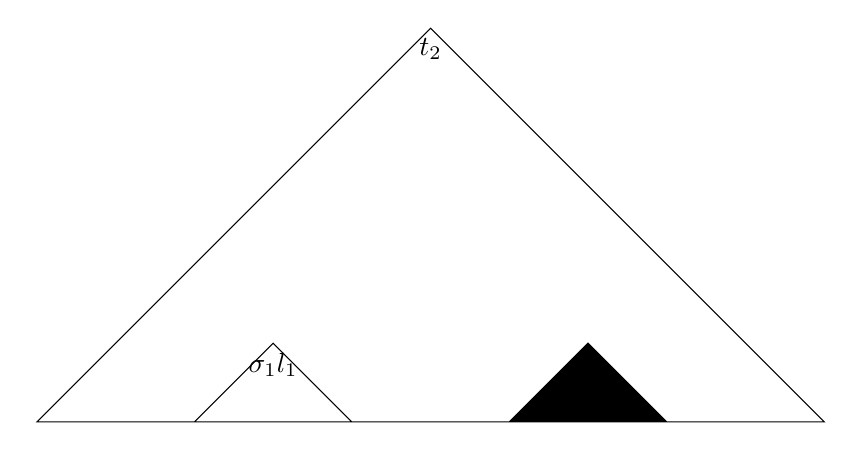
\begin{tikzpicture}
\node(a) at (8,0) {};
\node (b) at (6,0) {};
\node (c) at (7,1) {};

\draw (0,0) node[anchor=north]{}
  -- (10,0) node[anchor=north]{}
  -- (5,5) node[below]{$t_2$}
  -- cycle
   (2,0) node[anchor=north]{}
  -- (4,0) node[anchor=north]{}
  -- (3,1) node[below]{$\sigma_1 l_1$}
  -- cycle

  
     (8,0) node[anchor=north]{}
  -- (6,0) node[anchor=north]{}
  -- (7,1) node[below]{}
  -- cycle
  ;
\fill (a.center) -- (b.center) -- (c.center);

\end{tikzpicture}

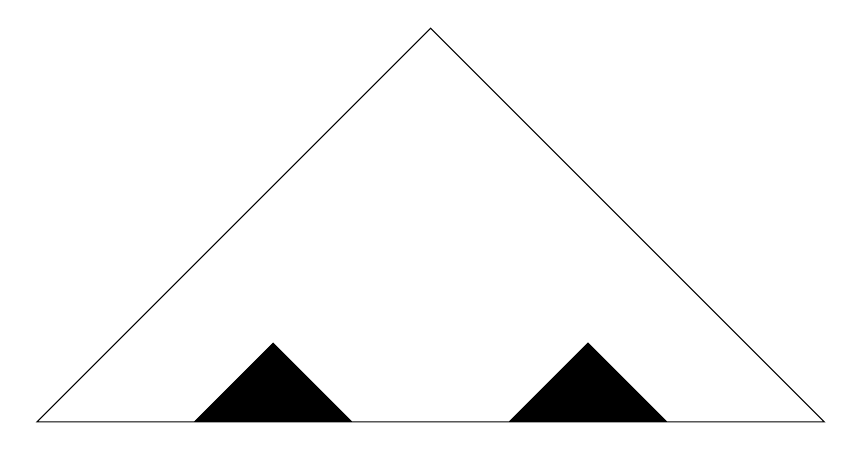
\begin{tikzpicture}
\node(a) at (8,0) {};
\node (b) at (6,0) {};
\node (c) at (7,1) {};
\node(a2) at (2,0) {};
\node (b2) at (4,0) {};
\node (c2) at (3,1) {};
\draw (0,0) node[anchor=north]{}
  -- (10,0) node[anchor=north]{}
  -- (5,5) node[below]{}
  -- cycle
   (2,0) node[anchor=north]{}
  -- (4,0) node[anchor=north]{}
  -- (3,1) node[below]{}
  -- cycle

  
     (8,0) node[anchor=north]{}
  -- (6,0) node[anchor=north]{}
  -- (7,1) node[below]{}
  -- cycle
  ;
\fill (a.center) -- (b.center) -- (c.center);
\fill (a2.center) -- (b2.center) -- (c2.center);
\end{tikzpicture}
  
\item Caso 2, $p_1$ es un prefijo de $p_2$

  \usetikzlibrary{decorations.pathreplacing}
\begin{tikzpicture}

\draw[dotted](5,3)--(10,3);
\draw[dotted](5,1)--(10,1);

\draw [decorate,decoration={brace,amplitude=10pt,mirror,raise=4pt},yshift=0pt]
(10,1) -- (10,3) node [black,midway,xshift=0.8cm] {\footnotesize
$p_1$};


\draw [decorate,decoration={brace,amplitude=10pt,mirror,raise=4pt},yshift=0pt]
(10,0) -- (10,1) node [black,midway,xshift=0.8cm] {\footnotesize
$p$};

\draw [decorate,decoration={brace,amplitude=10pt,mirror,raise=4pt},yshift=0pt]
(11,0) -- (11,3) node [black,midway,xshift=0.8cm] {\footnotesize
$p_2$};


\draw (0,0) node[anchor=north]{}
  -- (10,0) node[anchor=north]{}
  -- (5,5) node[below]{$s$}
  -- cycle
   (2,0) node[anchor=north]{}
  -- (8,0) node[anchor=north]{}
  -- (5,3) node[below]{$\sigma_1 l_1$}
  -- cycle

  
     (4,0) node[anchor=north]{}
  -- (6,0) node[anchor=north]{}
  -- (5,1) node[below]{$\sigma_2 l_2$}
  -- cycle
  ;

\end{tikzpicture}

\item Caso 3

  \usetikzlibrary{decorations.pathreplacing}
\begin{tikzpicture}

\draw[dotted](8,2)--(10,2);
\draw[dotted](5,1)--(10,1);
\draw[dotted](5,5)--(10,5);
\draw(2,2)--(8,2);

\draw [decorate,decoration={brace,amplitude=10pt,mirror,raise=4pt},yshift=0pt]
(10,1) -- (10,3) node [black,midway,xshift=0.8cm] {\footnotesize
$p_1$};


\draw [decorate,decoration={brace,amplitude=10pt,mirror,raise=4pt},yshift=0pt]
(10,0) -- (10,1) node [black,midway,xshift=0.8cm] {\footnotesize
$p$};

\draw [decorate,decoration={brace,amplitude=10pt,mirror,raise=4pt},yshift=0pt]
(11,0) -- (11,3) node [black,midway,xshift=0.8cm] {\footnotesize
$p_2$};


\draw (0,0) node[anchor=north]{}
  -- (10,0) node[anchor=north]{}
  -- (5,5) node[below]{$l_1$}
  -- cycle
  
     (4,0) node[anchor=north]{}
  -- (6,0) node[anchor=north]{}
  -- (5,1) node[below]{$\sigma_2 l_2$}
  -- cycle
  ;

\end{tikzpicture}
  
\end{itemize}




\begin{defi}
  Sea $l_i \rightarrow r_i$, $i = 1,2$ dos reglas cuyas variables han
  sido renombradas tal que
  $\Var(l_1,r_1) \cap \Var(l_2,r_2) = \emptyset$. Sea
  $p \in \Pos(l_1)$ tal que $l_1|_p$ no es una variable, y $\theta$ un
  umg de $l_1|_p =^? l_2$. Esto determinará el par crítico $\langle
  \theta r_1, (\theta l_1) [\theta r_2 ]_p \rangle$.
  % DIBUJO DEL ARBOL
  Si dos reglas dan lugar a un par crítico, diremos que se solapan.
\end{defi}

% EJEMPLO

A continuación enunciamos el Teorema de los Pares Críticos.
\begin{teor}
  Un sistema de reescritura es localmente confluente syss todos sus
  pares críticos se vuelven a unir.
\end{teor}

\begin{demo}
  ($\Leftarrow$) Sabemos que si $s \rightarrow_R t$ para $i = 1,2$,
  entonces es localmente confluente, ó $t_i = s[u_i]_p$, donde
  $\langle u_1, u_2 \rangle$ proviene de algún par crítico
  $\langle v_1, v_2 \rangle$, es decir $u_1 = \delta v_i$. Entonces
  $\xrightarrow{*}t$ para algún término, y por tanto
  $u_i \xrightarrow \delta t$ es tambień cierto. Esto implica
  $t_i \xrightarrow s[\delta t]_p$ para $i = 1,2$.

  ($\Rightarrow$) Como el sistema de reescritura es localmente
  confluente, esto significa que cuando lleguemos a un par crítico
  este volvera a converger a un término. Luego todos sus pares
  críticos se vuelven a unir.
\end{demo}

Algunas propiedades directas de este teorema,

\begin{coro}\label{parcritcor}
  Un sistema de términos terminante es confluente syss todos sus pares
  críticos se vuelven a unir
\end{coro}

Pero si además pedimos que sea un sistema finito, obtenemos el
siguiente resultado.

\begin{coro}
  La confluencia de un sistema de reescritura finito y terminante es
  decidible.
\end{coro}

\begin{demo}
  El algorítmo que seguiremos será el siguiente:

  Para cada par de reglas $l_1 \rightarrow r_1$ y
  $l_2 \rightarrow r_2$, y para cada $p \in \Pos(l_1)$, tal que
  $l_1|_p$ no es una variable, se genera un par crítico unificando las
  variables disjuntas de $l_1|_p$ y $l_2$.

  Para cada uno de esos pares críticos $\langle u_1, u_2 \rangle$
  reducimos $u_i$ a su forma normal $\tilde{u}_i$. Decimos que el
  sistema de reescritura es confluente syss
  $\tilde{u}_1 = \tilde{u}_2$ para todos sus pares críticos.

  Si se verifica $\tilde{u}_1 = \tilde{u}_2$, entonces por el
  corolario \ref{parcritcor}, el sistema es confluente.

  Si se da el caso de que existe algún par crítico no
  $\tilde{u}_1 \not = \tilde{u}_2$, entonces se da la situación
  $\tilde{u}_1 \xleftarrow{*} u_1 \leftarrow u \rightarrow u_2
  \xrightarrow{*} \tilde{u_2}$, que demostraría que no es confluente.
\end{demo}

\section{Implementación de los pares críticos}

Se implementarán una función para calcular los pares críticos. Antes
de poder definirla, se necesitarán varias funciones auxiliares. El
código se puede encontrar en el fichero \texttt{ParesCriticos.hs}.

Vamos a necesitar la librería de términos.
\begin{codigo}
import Terminos
\end{codigo}

\begin{itemize}
\item \texttt{(indiceMaximo t)} es el mayor índice que aparece en
  \texttt{t}. Por ejemplo,
\begin{sesion}
ghci> indiceMaximo (V ("x",3))
3
ghci> indiceMaximo (T "w" [V("x",4), V("z", 200), V("y", 1)])
200
\end{sesion}

Su código es,

\begin{code}
indiceMaximo :: Termino -> Indice
indiceMaximo (V (_,i)) = i
indiceMaximo (T _ ts) = maximum (map indiceMaximo ts)
\end{code}

\item \texttt{(renombraTermino n t)} es el termino resultante tras sumar a
  todos los índices de \texttt{t} el entero \texttt{n}. Por ejemplo,
\begin{sesion}
ghci> renombraTermino 5 (V ("x",3)) 
V ("x",8)
ghci> renombraTermino 3 (T "w" [V("x",4), V("z", 200), V("y", 1)])
T "w" [V ("x",7),V ("z",203),V ("y",4)]
\end{sesion}

Su código es,

\begin{codigo}
renombraTermino :: Int -> Termino -> Termino
renombraTermino n (V (x,i)) = V(x,i+n)
renombraTermino n (T f ts) = T f (map (renombraTermino n) ts)
\end{codigo}

\item \texttt{(parCritico c l1 r1 l2 r2)} calcula el par crítico de la
  regla $\texttt{l1} \rightarrow \texttt{r1}$ y
  $\texttt{l2} \rightarrow \texttt{r2}$. Por ejemplo,

% FALTA CP y CPS
\end{itemize}
    


%%%%%%%%%%%%%%%%%%%%%%%%%%%%%%%%%%%%%%%%%%%%%%%%%%%
%%Apéndices
%%%%%%%%%%%%%%%%%%%%%%%%%%%%%%%%%%%%%%%%%%%%%%%%%%%

\clearpage
\addappheadtotoc
\appendix


%%% Local Variables:
%%% mode: latex
%%% TeX-master: "SRT_en_Haskell"
%%% End:
